% Layout 1
\documentclass[a4paper, pdftex, ngerman, 11pt]{article}

\usepackage[utf8]{inputenc}
\usepackage[T1]{fontenc}
\usepackage{babel}
\usepackage{lmodern}

%%   linker Seitenabstand 4,5cm, rechter Seitenabstand 3,5cm und Abstand zum Seitenbeginn 2,5cm   %%
\usepackage[left=45mm,right=35mm,top=25mm,bottom=25mm]{geometry}
%%   Schriftart Arial   %%
\usepackage{helvet}
\renewcommand\familydefault{phv}
%%   1,3-facher Zeilenabstand   %%
\usepackage{setspace}
\setstretch{1.3}
%%   selbstdefinierte Kopf- und Fusszeile   %%
\usepackage{fancyhdr}
\pagestyle{fancy}
\fancyhead[L]{Fachschaft WIAI}
\fancyhead[C]{Otto-Friedrich Universität}
\fancyhead[R]{\today}
\fancyfoot[L]{}
\fancyfoot[C]{\thepage}
\fancyfoot[R]{}
%  Breite der Linie unter der Kopfzeile 
\renewcommand{\headrulewidth}{0pt}


%%   Einbidung der Farben und -definitionen des vordefinierten Farbschemas   %%
\usepackage{color}
\definecolor{darkred}{rgb}{.5,0,0}
\definecolor{darkgreen}{rgb}{0,.5,0}
\definecolor{darkblue}{rgb}{0,0,.5}
\usepackage[hyphens]{url}

%%   Zur Gestaltung des Textes zu einem Hypertext   %%
\usepackage{hyperref}
%\definecolor{darkblue}{rgb}{0,.05,.54}
\hypersetup{colorlinks=true, breaklinks=true, linkcolor=darkblue, menucolor=darkblue, urlcolor=darkblue, citecolor=darkblue, filecolor=darkblue}
\urlstyle{same}

\usepackage{longtable}
\usepackage{graphicx}
\usepackage{float}
\usepackage{listings}

\begin{document}
% Layout 1 - Titelseite
%\begin{titlepage}
\begin{center}
\Huge \LaTeX\\
\vspace{5mm} \LARGE Eine kurze Einführung\\
\vspace{12mm} \Large  Universität Bamberg\\[5mm]
\large 08. April 2015\\
Fachschaft WIAI\normalsize \\
\end{center}
%\end{titlepage}

%%   Seitennummerierung mit roemischer Nummerierung   %%
\pagenumbering{Roman}
%%   Beginne die Seitennummerierung mit 2 ab dem Inhaltsverzeichnis   %%
\setcounter{page}{2}
\tableofcontents
\newpage
\listoffigures
\newpage
\listoftables
\newpage
%%   Hauptteil   %%
%%   Seitennummerierung mit arabischer Nummerierung   %%
\pagenumbering{arabic}
%%   Beginne die Seitennummerierung mit 1 ab dem ersten eingebunden Dokument   %%
\setcounter{page}{1}
\section{$\mathcal{A}2$} 
\begin{frame}
\frametitle{Aufgabe 2}
\framesubtitle{Baut Aufgabe2.pdf mit \LaTeX ~nach!} 

\begin{block}{\"Ubung 2}
\begin{itemize}
  \item Benennt Eure Dateien einheitlich
  \item Verwendet passende Abschnittsbefehle
  \item Wenn was schief l\"auft, schaut in der Konsole nach
  \item \"Ubung macht den Meister!
\end{itemize}
\end{block}
\end{frame}
\newpage
\section{Warum heißt der Pinguin "`Pinguin"'?}
\subsection{Erklärung 1}
Ursprünglich kommt der Name aus dem walisischen und heißt dort 'Pen Gwyn' (gesprochen wie das englische penguin). Es bedeutet soviel wie 'Weisser Kopf'. Seeleute aus Wales sollen die Tiere als erste gesehen und so genannt haben (siehe dazu Bild \ref{img:pen}).

\begin{figure}[H]
\begin{center}

\includegraphics[width=4cm]{bilder/swim-Ping.jpg}
\caption{Ein lebendes Exemplar eines Pinguins}
\label{img:pen}
\end{center}
\end{figure}

\subsection{Erklärung 2}
Es heißt aber auch, da\ss \ ursprünglich der Name 'Pinguin' eine Bezeichnung für den 1844 ausgestorbenen, ebenfalls flugunfähigen Riesenalk der Nordhalbkugel war (siehe Bild \ref{img:auk}).

\begin{figure}[H]
\begin{center}
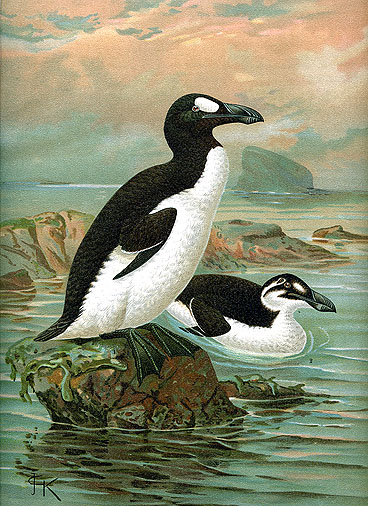
\includegraphics[width=5cm]{bilder/GreatAuk.jpg}
\caption{Ein besonders pr"achtiges Exemplar eines Pinguins}
\label{img:auk}
\end{center}
\end{figure}

\subsection{Erklärung 3}
Eine andere These lautet, dass der Name vom lateinischen "`penguis"' stammt. Dies bedeutet "`Fett"' und für die Seefahrer war Fett sehr wichtig und es ließ sich aus den Pinguinen gewinnen (siehe Bild \ref{img:tux}).

\begin{figure}[H]
\begin{center}

\includegraphics[width=5cm]{bilder/tux.png}
\caption{Der kleine Tux}
\label{img:tux}
\end{center}
\end{figure}

\newpage
\documentclass[a4paper, pdftex, ngerman, 11pt]{article}
%IMMER!!!
\usepackage[utf8]{inputenc}
\usepackage[T1]{fontenc}
\usepackage{babel}
\usepackage[iso]{umlaute}

\usepackage{longtable}
\usepackage{listings}
\usepackage{color}

\begin{document}
\section{Aufgabe 4}
\subsection{Tabellen \& Formeln}
Die Tabelle \ref{tab:ani} besteht aus 3 Spalten:\\
Die erste Spalte ist mit einem p von 25mm definiert. Die zweite und die dritte Spalte sind zentriert.

\begin{longtable}{p{25mm}|c|c}
& Fuchs & Elster\\
\hline
\hline
Familie & Hunde & Rabenvögel\\
\hline
Gewicht & m: 6,6kg w: 5,5kg & 200--250g\\
\hline
Geschwindigkeit $ = \sqrt{v\cdot v}$ & $55\frac{km}{h}$ & mind. superschnell: $\lim\limits_{x \rightarrow \infty} x \cdot v$ \\
\hline
Farbe & tödlich & schwarz\\
\hline
\caption{Wild Animals}
\label{tab:ani}
\end{longtable}

Der Sinn des Lebens$^2$: $\prod\limits_{i=1}^{n+1} i + \sum_{j=0}^{n} j \cdot \int\limits_{\pi}^{Daumen} 42$

\subsection{Aufzählungen}
Um bei den vielen Verschachtelungen nicht den Überblick zu verlieren, sind Einrückungen der items sinnvoll.
\begin{enumerate}
  \item 
  \begin{enumerate}
    \item Vorteile des Fuchses:
    \item
    \begin{itemize}
      \item schlau
      \item schaut cool aus
    \end{itemize}
    \item Nachteile des Fuchses:
    \begin{itemize}
      \item Pelz wird verarbeitet
      \item sehr viele Autos fahren gerne über Füchse
    \end{itemize}
    \item Spam Spam Spam
  \end{enumerate}
  \item
  \begin{enumerate}
    \item Vorteile der Elster...
    \item Nachteile der Elster:
    \begin{itemize}
      \item Diebischkeit wird bestraft
      \item viele landen hinter Gittern
    \end{itemize}
      \item singt ganz gut, aber ist gefährlich
  \end{enumerate}
\end{enumerate}

\subsection{(Un)Logik}
\begin{itemize}
	\item $\lnot\forall x \Leftrightarrow \{\exists x\}$
	\item $[\exists xPx] \rightarrow \forall x \lnot Px$
\end{itemize}

\subsection{Code}
\textit{Hello World} in Java:\\
\lstset{language=Java, commentstyle=\color{green}}
\begin{lstlisting}
  public class Hello{
      public static void main(String[] args){
      
         //Hier wird der Text ausgegeben:
         System.out.println("Hello World!");
      }
  }
\end{lstlisting}

\end{document}

\textbf{Herzlichen Gl"uckwunsch, du hast das \LaTeX -Tutorium der Fachschaft WIAI bis zum Ende geschafft!}
\end{document}
